\documentclass[9pt]{beamer}
\mode<presentation>

% Tema e Cores (Conforme original)
\usetheme{Madrid}
\usepackage{xcolor}
\definecolor{mGreen}{rgb}{0,0.6,0}
\definecolor{mRed}{rgb}{0.6,0,0}
\usecolortheme[RGB={0,100,50}]{structure}
\usefonttheme{structurebold} 
\setbeamercovered{invisible} 

% Pacotes Adicionais
\usepackage{dynblocks}
\usepackage{textpos}
\usepackage{amsfonts, amsmath, amssymb, amsthm}
\usepackage{listings}
\usepackage{tikz}
\usepackage{pgfplots}
\pgfplotsset{compat=1.18}
\usepackage{mathtools}
\usepackage[portuguese]{babel}
\usepackage{hyperref}
\usepackage[utf8]{inputenc}
\usepackage[T1]{fontenc}
\usepackage{lmodern}
\usepackage[pscoord]{eso-pic}
\usepackage{listings}
\usepackage{xcolor}
\usetikzlibrary{shapes,arrows,positioning, calc}

% Configurações de Título
\title[SRE Monitoring]{Engenharia de Confiabilidade do Google (SRE)}
\subtitle{Monitoração Agregada e Princípios Fundamentais}
\author[Sergio Souza Novak]{Professor: Me. Sergio Souza Novak}
\institute[UniRV]{Faculdade de Engenharia de Software \\ Universidade de Rio Verde}
\date{}

\titlegraphic{
\includegraphics[width=4cm]{Universidade_de_Rio_Verde.jpg}}

\begin{document}

% -------------------------------------------------------
% Título
% -------------------------------------------------------
\frame[plain]{\titlepage}

\AddToShipoutPictureFG{
    \put(\LenToUnit{.92\paperwidth},
    \LenToUnit{.185\paperheight})
    {\vtop{{\null}
    \makebox{
\includegraphics[width=.8cm,keepaspectratio]{Universidade_de_Rio_Verde.jpg}}}}}

% -------------------------------------------------------
% Sumário
% -------------------------------------------------------
\begin{frame}{Sumário}
  \tableofcontents
\end{frame}

% -------------------------------------------------------
% SEÇÃO 1: INTRODUÇÃO
% -------------------------------------------------------
\section{Introdução à Monitoração SRE}

\begin{frame}{Definição de Monitoração no Google}
\begin{block}{O que é monitoração?}
Coleta, processamento, agregação e visualização de dados quantitativos em tempo real sobre um sistema.
\end{block}
\begin{figure}
\centering
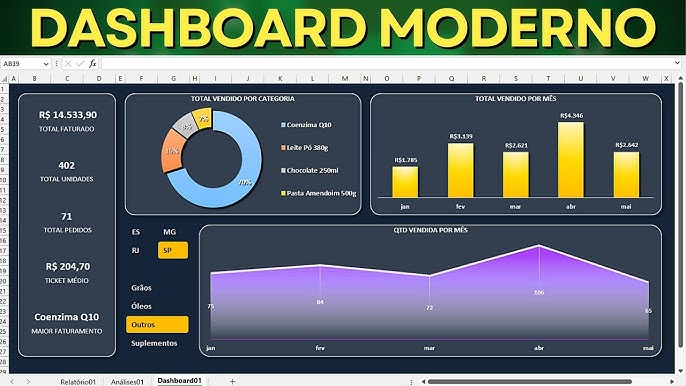
\includegraphics[width=0.2\linewidth]{hq720.jpg}
\caption{Dashboard}
\end{figure}
\begin{itemize}
    \item \textbf{Visibilidade:} Saber se o sistema está "vivo".
    \item \textbf{Análise:} Entender o comportamento sob carga.
    \item \textbf{Resposta:} Atuar proativamente antes da falha total.
\end{itemize}

\begin{alertblock}{Princípio SRE}
Se você não consegue medir, você não consegue gerenciar nem melhorar a confiabilidade.
\end{alertblock}
\end{frame}

\begin{frame}{Definição de Monitoração no Google}
\begin{figure}
\centering
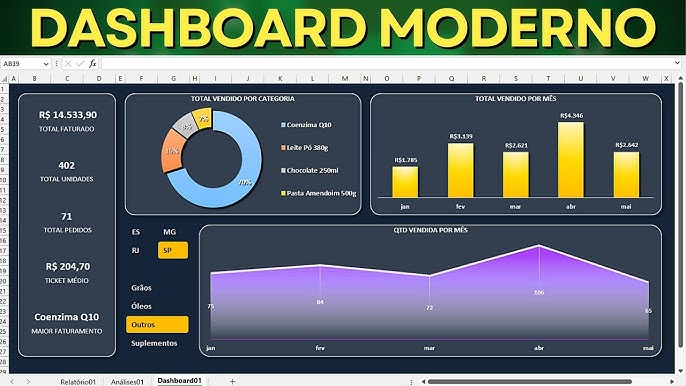
\includegraphics[width=\linewidth]{hq720.jpg}
\caption{Dashboard}
\end{figure}

\end{frame}
\begin{frame}{Dashboard Kubernetes}
\begin{figure}
\centering
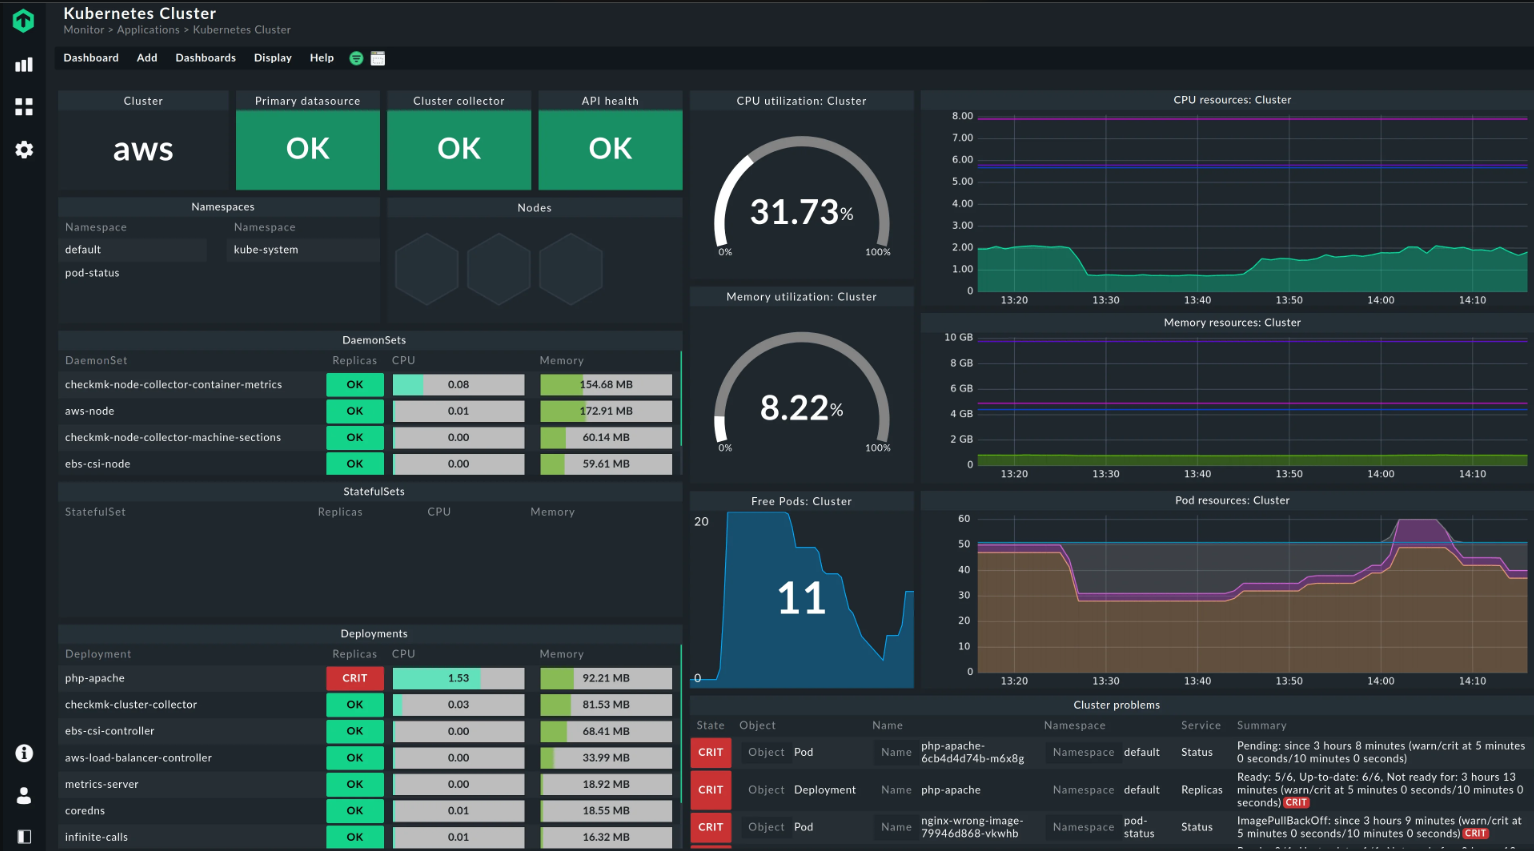
\includegraphics[width=\linewidth]{dashboard_kubernetes.png}
\caption{Dashboard}
\end{figure}

\end{frame}
\begin{frame}{Dashboard Itaipú}
\begin{figure}
\centering
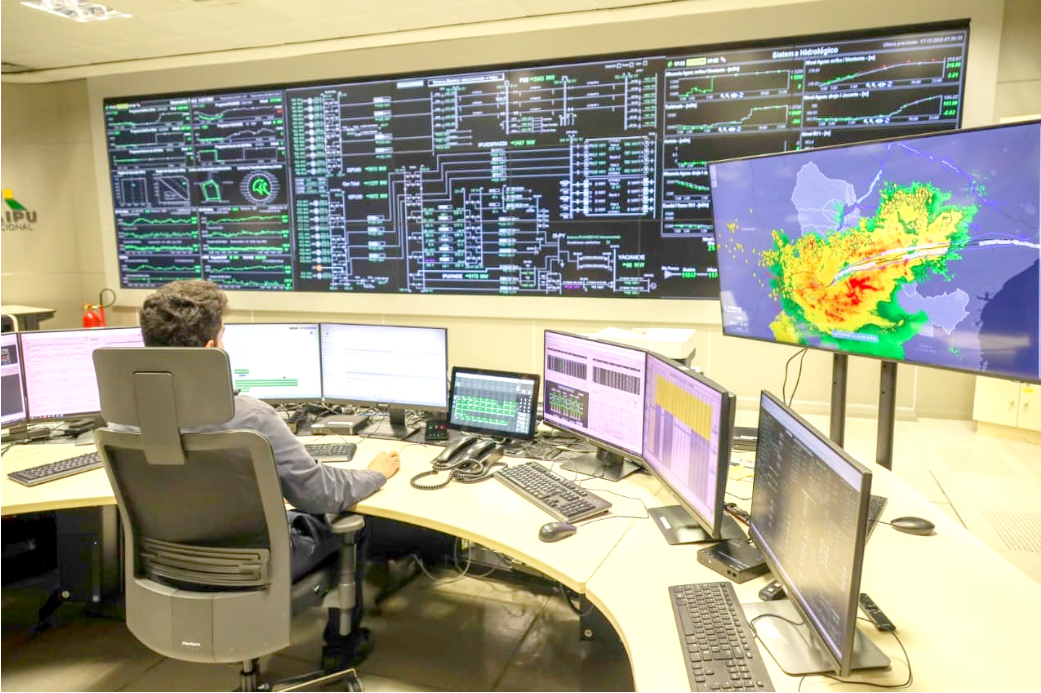
\includegraphics[width=\linewidth]{dashboard_itaipu.png}
\caption{Dashboard}
\end{figure}

\end{frame}
\begin{frame}{Monitoração}
\begin{figure}
\centering

\begin{minipage}{0.25\linewidth}
\centering
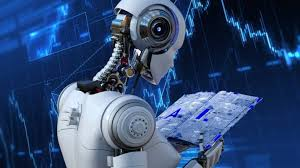
\includegraphics[width=\linewidth]{interpretacao_robo.jpeg}
\caption{Interpretação automática por software}
\end{minipage}
\begin{minipage}{0.25\linewidth}
\centering 
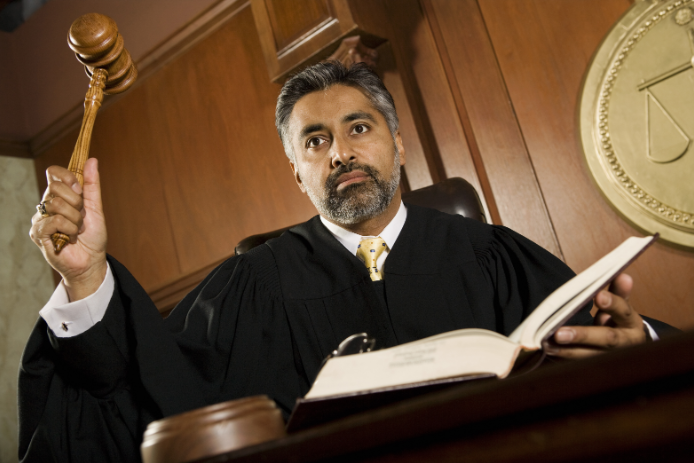
\includegraphics[width=\linewidth]{juiz.png}
\caption{Interpretação humana}
\end{minipage}

\end{figure}
\begin{block}{Definição}
A monitoração é um mecanismo utilizado para acompanhar a
\textbf{saúde} e a \textbf{disponibilidade} de um sistema ao longo do tempo.
\end{block}

\begin{alertblock}{Problema da abordagem tradicional}
Um sistema que exige que uma pessoa leia um email e interprete
manualmente um alerta possui uma falha fundamental.
\end{alertblock}

\begin{block}{Boa prática}
A interpretação dos eventos deve ser realizada por \textbf{software}.
Os seres humanos devem ser notificados apenas quando
\textbf{uma ação precisa ser tomada}.
\end{block}

\end{frame}
\begin{frame}{Saída de Monitoração: Alertas}
\begin{figure}
\centering
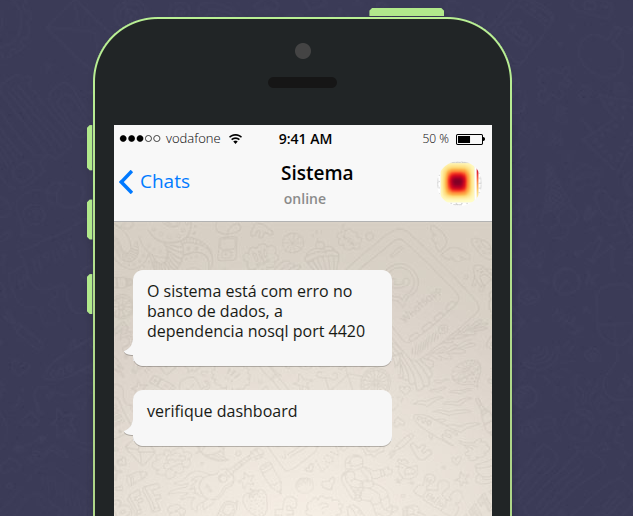
\includegraphics[width=\linewidth]{alert.png}
\caption{Alerta}
\end{figure}


\end{frame}
\begin{frame}{Saída de Monitoração: Alertas}
\begin{figure}
\centering
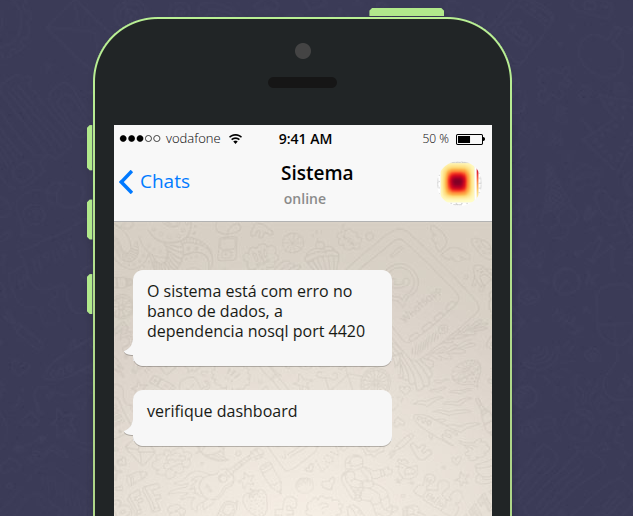
\includegraphics[width=0.2\linewidth]{alert.png}
\caption{Alerta}
\end{figure}

\begin{alertblock}{Alertas}
Indicam que um ser humano deve tomar uma \textbf{ação imediata}
para evitar ou resolver um problema crítico no sistema.
\end{alertblock}

\begin{block}{Exemplos}
\begin{itemize}
\item Servidor fora do ar
\item Banco de dados indisponível
\item Uso extremo de CPU ou memória
\end{itemize}
\end{block}

\end{frame}
\begin{frame}{Saída de Monitoração: Tickets}
\begin{figure}
\centering
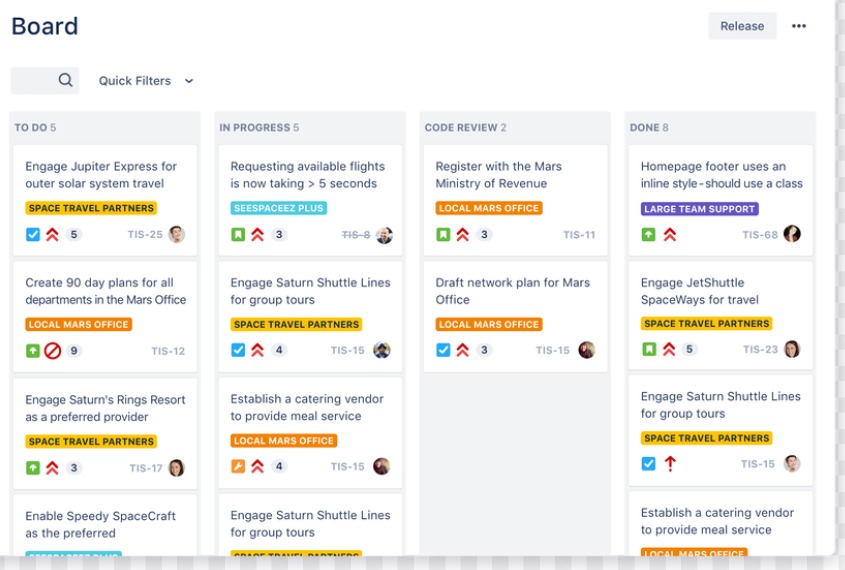
\includegraphics[width=\linewidth]{ticket.png}
\caption{Ticket}
\end{figure}
\end{frame}

\begin{frame}{Saída de Monitoração: Tickets}

\begin{block}{Tickets}
Indicam que uma ação humana será necessária, porém
\textbf{não imediatamente}.
\end{block}

\begin{alertblock}{Interpretação}
O sistema não consegue resolver o problema automaticamente,
mas existe tempo suficiente para que a situação seja tratada
posteriormente sem causar danos.
\end{alertblock}

\begin{block}{Exemplos}
\begin{itemize}
\item Disco com alto nível de utilização
\item Atualização de software necessária
\item Manutenção preventiva
\end{itemize}
\end{block}

\end{frame}
\begin{frame}{Saída de Monitoração: Logging}

\begin{block}{Logging}
Consiste no registro de eventos do sistema para
\textbf{diagnóstico, auditoria e investigação}.
\end{block}

\begin{alertblock}{Característica}
Essas informações normalmente não precisam ser analisadas
imediatamente por um ser humano.
\end{alertblock}

\begin{block}{Exemplos}
\begin{itemize}
\item Registro de acessos ao sistema
\item Histórico de erros
\item Logs de operações executadas
\end{itemize}
\end{block}

\end{frame}
\begin{frame}{Saída de Monitoração: Logs}
\begin{figure}
\centering
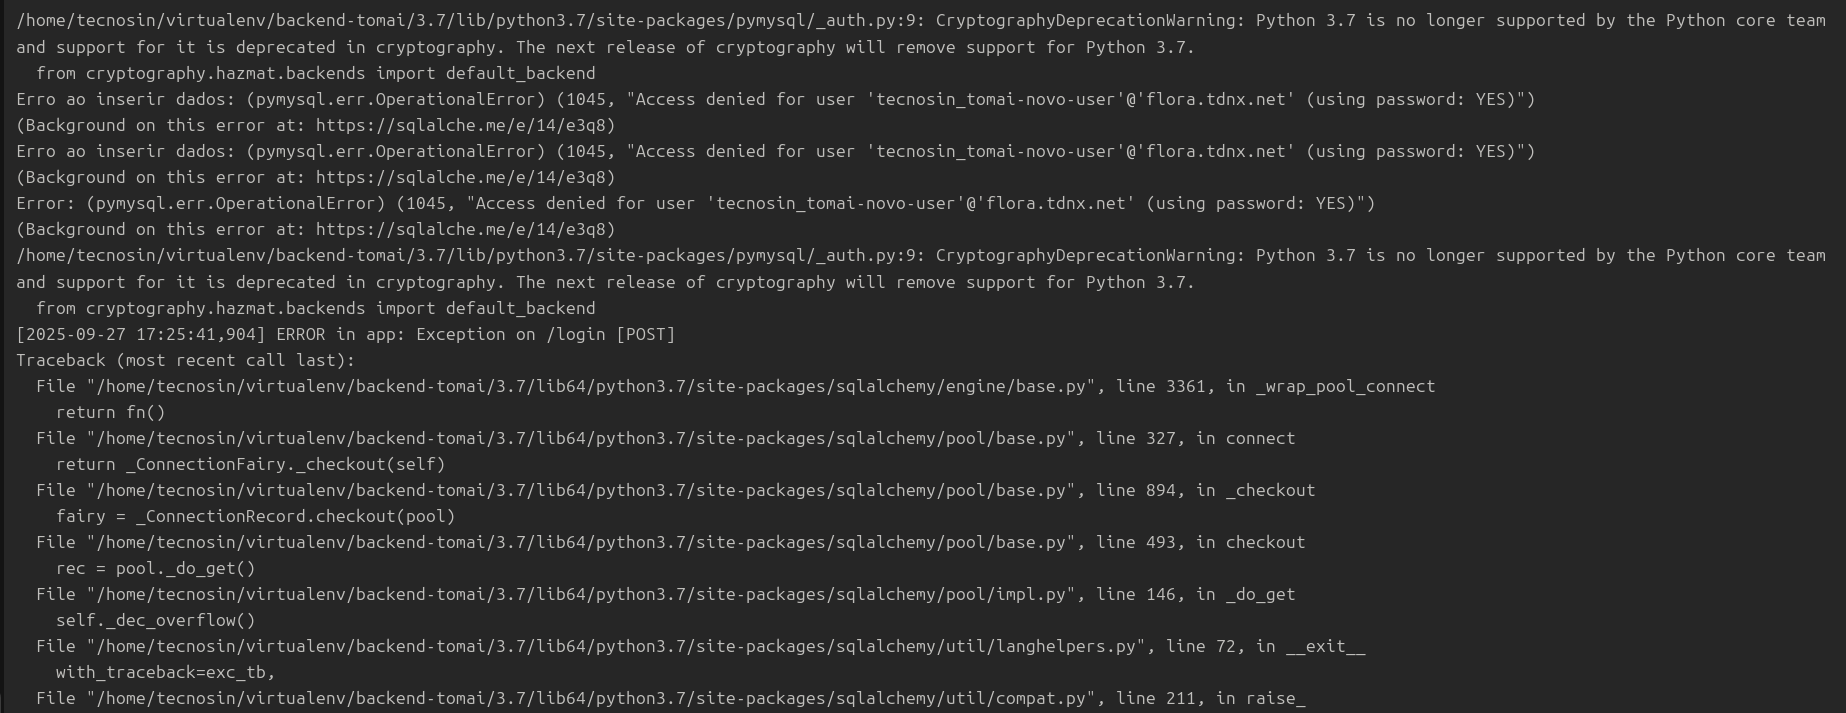
\includegraphics[width=\linewidth]{log.png}
\caption{Log}
\end{figure}
\end{frame}

\begin{frame}{Por que monitorar?}
\begin{itemize}
    \item \textbf{Alertas:} Notificar quando há problemas que exigem intervenção humana.
    \item \textbf{Depuração (Debugging):} Fornecer contexto para encontrar a causa raiz.
    \item \textbf{Análise de Longo Prazo:} Identificar tendências de uso e capacidade.
    \item \textbf{Dashboarding:} Visualização rápida de saúde para stakeholders.
\end{itemize}
\end{frame}

\begin{frame}{Hierarquia de Necessidades de Confiabilidade}
\begin{center}
\begin{tikzpicture}
\coordinate (A) at (0,0);
\coordinate (B) at (4,0);
\coordinate (C) at (2,3.5);
\draw[thick, fill=structure!10] (A) -- (B) -- (C) -- cycle;

\node at (2,0.4) {\footnotesize Monitoração};
\node at (2,1.2) {\footnotesize Resposta Incidentes};
\node at (2,2.0) {\footnotesize Post-mortems};
\node at (2,2.8) {\footnotesize Produto};

\draw (0.5,0.8) -- (3.5,0.8);
\draw (1.0,1.6) -- (3.0,1.6);
\draw (1.5,2.4) -- (2.5,2.4);
\end{tikzpicture}
\end{center}
\begin{block}{Monitoração é a Base}
Todo o trabalho de SRE (Resposta, Mudança, Capacidade) depende de dados sólidos de monitoração.
\end{block}
\end{frame}

% -------------------------------------------------------
% SEÇÃO 2: TIPOS DE MONITORAÇÃO
% -------------------------------------------------------
\section{White-box vs. Black-box}

\begin{frame}{Monitoração de "Caixa-Preta" (Black-box)}
\begin{block}{Foco no Sintoma Externo}
Observa o sistema de fora, simulando a experiência do usuário final.
\end{block}
\begin{itemize}
    \item \textbf{Vantagem:} Descobre se o serviço está quebrado \textit{agora}.
    \item \textbf{Desvantagem:} Não explica \textit{por que} está quebrado.
    \item \textbf{Uso Típico:} Paging (Alertas críticos de disponibilidade).
\end{itemize}
\end{frame}

\begin{frame}{Monitoração de "Caixa-Branca" (White-box)}
\begin{block}{Foco no Interior}
Métricas expostas pela própria aplicação: logs, contadores, estados de CPU, latência interna.
\end{block}
\begin{itemize}
    \item \textbf{Vantagem:} Permite monitorar componentes internos que ainda não falharam externamente.
    \item \textbf{Diagnóstico:} Essencial para depurar problemas de performance e gargalos silenciosos.
    \item \textbf{Fonte:} Instrumentação de código (Ex: Prometheus, Stackdriver).
\end{itemize}
\end{frame}

\begin{frame}{Comparação: Quando Usar cada Uma?}
\begin{table}
\centering
\begin{tabular}{|l|p{3.5cm}|p{3.5cm}|}
\hline
\textbf{Atributo} & \textbf{Black-box} & \textbf{White-box} \\ \hline
Visão & Externo/Usuário & Interno/Código \\ \hline
Propósito & Alerta de crise & Depuração/Capacidade \\ \hline
Sensibilidade & Alta (impacto direto) & Muito Alta (m detalhes) \\ \hline
\end{tabular}
\end{table}
\begin{exampleblock}{Regra de Ouro}
Use Black-box para saber \textit{o quê} está errado. Use White-box para saber \textit{onde} está o erro.
\end{exampleblock}
\end{frame}

% -------------------------------------------------------
% SEÇÃO 3: OS 4 SINAIS DE OURO
% -------------------------------------------------------
\section{Os 4 Sinais de Ouro}

\begin{frame}{1. Latência}
    \begin{figure}
\centering
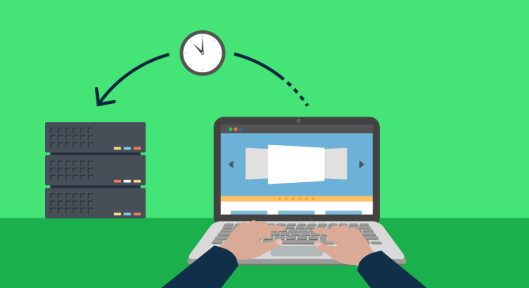
\includegraphics[width=0.6\linewidth]{latencia.png}
\end{figure}
\begin{block}{Definição}
O tempo que leva para atender a uma requisição.
\end{block}
\begin{itemize}
    \item \textbf{Atenção:} Monitore separadamente a latência das \textbf{requisições de sucesso} e das \textbf{requisições de erro}.
    \item \textit{Exemplo:} Um erro 500 rápido pode mascarar uma latência terrível em requisições de sucesso se você olhar apenas a média global.
\end{itemize}
\end{frame}

\begin{frame}{2. Tráfego}
    \begin{figure}
\centering
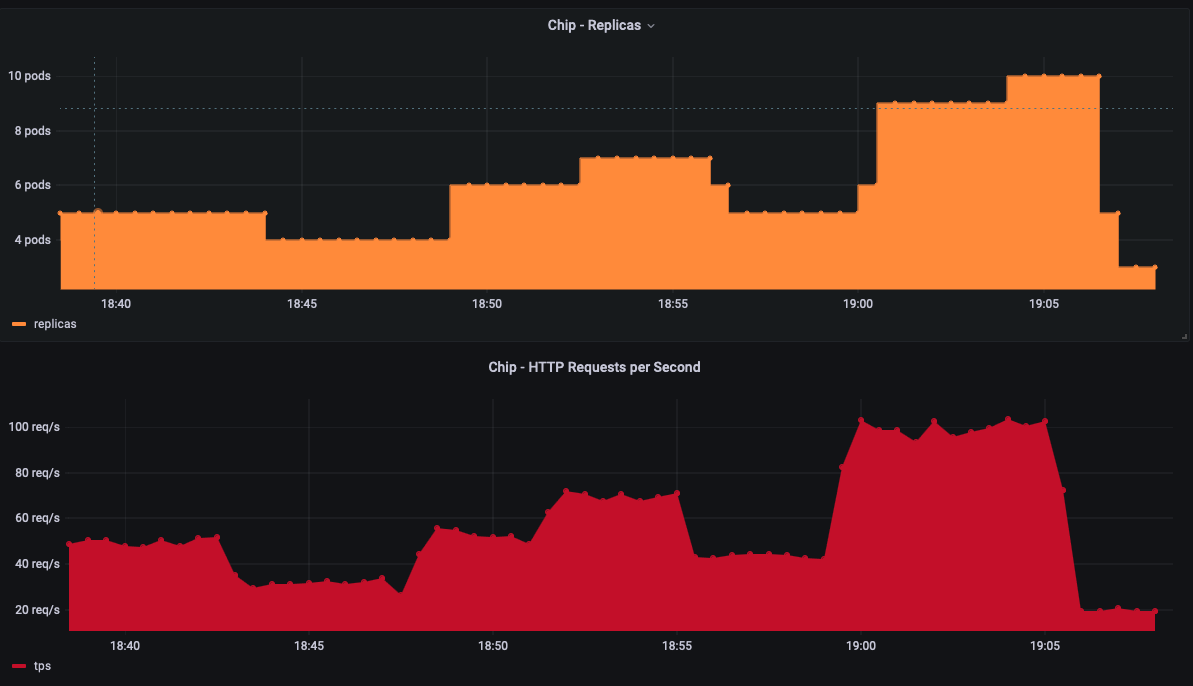
\includegraphics[width=0.6\linewidth]{tps-keda.png}
\end{figure}
\begin{block}{Definição}
A demanda que o sistema está recebendo.
\end{block}
\begin{itemize}
    \item \textbf{Sistemas HTTP:} Requisições por segundo (RPS).
    \item \textbf{Streaming:} Taxas de entrada/saída de dados.
    \item \textbf{Armazenamento:} I/O operations.
\end{itemize}
\end{frame}

\begin{frame}{3. Erros}
\begin{block}{Definição}
A taxa de requisições que falharam.
\end{block}
\begin{itemize}
    \item \textbf{Explícitos:} Status 500, timeouts.
    \item \textbf{Implícitos:} Resposta 200 que contém conteúdo de erro ou está vazia.
    \item \textbf{Incorretos:} O servidor configurou o código de retorno errado.
\end{itemize}
\end{frame}

\begin{frame}{4. Saturação}
\begin{block}{Definição}
Quão "cheio" está o sistema em relação aos seus recursos finitos.
\end{block}
\begin{itemize}
    \item \textbf{Métricas:} Memória, CPU, threads em espera, largura de banda.
    \item \textbf{Aviso:} Muitos sistemas sofrem degradação de performance muito antes de atingirem 100\% de saturação.
\end{itemize}
\end{frame}

\begin{frame}{Resumo dos 4 Sinais de Ouro}
\begin{center}
\begin{tikzpicture}[node distance=1.5cm]
\node (A) [draw, fill=mGreen!10, text width=2.5cm, align=center] {Latência};
\node (B) [draw, right=of A, fill=mGreen!10, text width=2.5cm, align=center] {Tráfego};
\node (C) [draw, below=of A, fill=mRed!10, text width=2.5cm, align=center] {Erros};
\node (D) [draw, right=of C, fill=mRed!10, text width=2.5cm, align=center] {Saturação};
\end{tikzpicture}
\end{center}
\end{frame}

% -------------------------------------------------------
% SEÇÃO 4: SLOs E ORÇAMENTO DE ERRO
% -------------------------------------------------------
\section{SLOs e Monitoração}

\begin{frame}{SLI — Service Level Indicator}
\begin{center}
\begin{tikzpicture}[node distance=3cm]

\node (user) [draw, rounded corners, fill=blue!10, text width=1.5cm, align=center]
{Usuário};

\node (system) [draw, rounded corners, fill=blue!10, right of=user, text width=2cm, align=center]
{Sistema / API};

\node (metric) [draw, rounded corners, fill=green!10, below of=system, text width=4cm, align=center]
{Métrica Observada \\ (SLI)};

\draw[->, thick] (user) -- node[above]{request} (system);
\draw[->, thick] (system) -- node[right]{tempo de resposta} (metric);

\end{tikzpicture}
\end{center}

\begin{block}{Definição}
\textbf{SLI (Service Level Indicator)} é uma métrica que mede o comportamento real do sistema.
\end{block}

\begin{itemize}
\item Latência de requisições
\item Taxa de erros
\item Disponibilidade do serviço
\end{itemize}

\end{frame}
\begin{frame}{SLO e SLA}
\begin{center}
\begin{tikzpicture}[node distance=2cm]

\node (sli) [draw, rounded corners, fill=green!15, text width=3cm, align=center]
{SLI \\ Métrica medida};

\node (slo) [draw, rounded corners, fill=yellow!20, below of=sli, text width=3.5cm, align=center]
{SLO \\ Meta de desempenho};

\node (sla) [draw, rounded corners, fill=red!15, below of=slo, text width=4cm, align=center]
{SLA \\ Acordo contratual};

\draw[->, thick] (sli) -- (slo);
\draw[->, thick] (slo) -- (sla);

\end{tikzpicture}
\end{center}

\begin{itemize}
\item \textbf{SLI:} Métrica observada no sistema.
\item \textbf{SLO:} Meta definida para essa métrica.
\item \textbf{SLA:} Consequências contratuais se o SLO não for cumprido.
\end{itemize}

\end{frame}
\begin{frame}{Orçamento de Erro (Error Budget)}

\begin{center}
\begin{tikzpicture}

\draw[fill=green!20] (0,0) rectangle (8,1);
\draw[fill=red!30] (7.2,0) rectangle (8,1);

\node at (3.5,0.5) {Disponibilidade esperada (99.9\%)};
\node at (7.6,0.5) {Erro (0.1\%)};

\end{tikzpicture}
\end{center}

\begin{block}{Conceito}
O orçamento de erro é a quantidade de falhas permitidas dentro do SLO.
\end{block}

\begin{itemize}
\item Se o SLO é \textbf{99.9\%}, então temos \textbf{0.1\% de falha permitida}.
\item Esse percentual é o \textbf{Error Budget}.
\item Se o orçamento acabar, novas mudanças devem parar para focar em estabilidade.
\end{itemize}

\end{frame}

\begin{frame}{Escolhendo Métricas Prioritárias}
\begin{itemize}
    \item Não monitore tudo com o mesmo rigor.
    \item Foque no que \textbf{gera valor para o usuário}.
    \item Evite métricas de "vaidade" (ex: número total de usuários logados não indica se o sistema está rápido).
\end{itemize}
\end{frame}

% -------------------------------------------------------
% SEÇÃO 5: FILOSOFIA DE ALERTAS
% -------------------------------------------------------
\section{Alertas e Ruído}

\begin{frame}{Classificação de Notificações}
\begin{enumerate}
    \item \textbf{Páginas (Alertas Instantâneos):} Acordam alguém. Use apenas para problemas críticos e resolvíveis.
    \item \textbf{Tickets:} Para problemas que precisam de ação, mas não urgentes.
    \item \textbf{Logs/Dashboards:} Para análise posterior ou tendência.
\end{enumerate}
\end{frame}
\begin{frame}{Alertas: Sintoma vs. Causa}

\begin{center}
\begin{tikzpicture}[node distance=3.8cm]

\node (cause) [draw, rounded corners, fill=red!15, text width=3cm, align=center]
{\textbf{Causa Interna} \\ Disco 80\%};

\node (symptom) [draw, rounded corners, fill=yellow!20, right of=cause, text width=3.2cm, align=center]
{\textbf{Sintoma} \\ Sistema lento};

\node (impact) [draw, rounded corners, fill=green!20, right of=symptom, text width=3.5cm, align=center]
{\textbf{Impacto no Usuário} \\ Emails falhando};

\draw[->, thick] (cause) -- (symptom);
\draw[->, thick] (symptom) -- (impact);

\node[above=0.4cm of cause] {\small Não alertar};
\node[above=0.4cm of impact] {\small \textbf{Alertar aqui}};

\end{tikzpicture}
\end{center}

\begin{alertblock}{Alerta baseado apenas na causa}
``Disco atingiu 80\%'' pode não causar nenhum problema real no serviço.
Isso gera muitos \textit{falsos alarmes}.
\end{alertblock}

\begin{exampleblock}{Alerta baseado no sintoma}
``20\% dos envios de e-mail estão falhando''.  
Isso indica impacto direto para os usuários e deve gerar alerta.
\end{exampleblock}

\end{frame}

\begin{frame}{Combatendo a Fadiga de Alertas}
\begin{itemize}
    \item Todo alerta deve ser \textbf{acionável}.
    \item Se você vê um alerta e ignora, a regra de alerta \textbf{deve ser removida}.
    \item Excesso de alertas irrelevantes esconde os reais incidentes.
\end{itemize}
\end{frame}

% -------------------------------------------------------
% SEÇÃO 6: MONITORAÇÃO AGREGADA
% -------------------------------------------------------
\section{Monitoração Agregada}

\begin{frame}{O Desafio da Escala}
    \begin{figure}
\centering
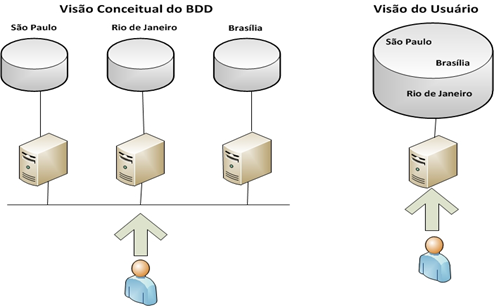
\includegraphics[width=0.5\linewidth]{sistema_distribuido1.png}
\end{figure}
Monitorar mil máquinas individualmente é impossível para humanos.
\begin{block}{Agregação}
Combine estatísticas de várias instâncias para ver o comportamento do \textit{cluster} como um todo.
\end{block}
\end{frame}
\section{Distribuilção de Dados e Percentis}

\begin{frame}{Distribuição de Frequência}

\begin{center}
\begin{tikzpicture}[scale=0.9]

\draw[->] (0,0) -- (7,0) node[right]{Valores};
\draw[->] (0,0) -- (0,4) node[above]{Frequência};

\draw[fill=blue!20] (0.5,0) rectangle (1.5,1.5);
\draw[fill=blue!20] (1.8,0) rectangle (2.8,3);
\draw[fill=blue!20] (3.1,0) rectangle (4.1,2.2);
\draw[fill=blue!20] (4.4,0) rectangle (5.4,1.2);
\draw[fill=blue!20] (5.7,0) rectangle (6.7,0.6);

\node at (3.5,-0.6){Classes de valores};

\end{tikzpicture}
\end{center}

\begin{block}{Definição}
A distribuição de frequência mostra quantas vezes valores aparecem em intervalos de uma variável.
\end{block}

Exemplo: alturas, pesos, latência de um sistema, tamanho de peixes.

\end{frame}
\begin{frame}{Percentis}

\begin{center}
\begin{tikzpicture}

\draw[->] (0,0) -- (10,0);

\draw (2,0) -- (2,0.5);
\node[below] at (2,0){P25};

\draw (5,0) -- (5,0.7);
\node[below] at (5,0){P50};

\draw (8,0) -- (8,0.5);
\node[below] at (8,0){P90};

\node at (5,1.2){Distribuição de dados};

\end{tikzpicture}
\end{center}

\begin{block}{Definição}
Um percentil indica a posição abaixo da qual uma porcentagem dos dados está.
\end{block}

Exemplo:

\begin{itemize}
\item P50 = mediana
\item P90 = 90\% dos dados estão abaixo desse valor
\end{itemize}

\end{frame}
\begin{frame}{Averages vs. Percentiles}
\begin{alertblock}{A Média mente!}
Em latência, a média esconde outliers. 
\end{alertblock}
\begin{itemize}
    \item Use **Percentis (P90, P95, P99)**.
    \item P99 de 1s significa que 1\% das requisições levaram mais de 1s.
    \item É aqui que os usuários "infelizes" estão escondidos.
\end{itemize}
\end{frame}

\begin{frame}{Distribuições :Assimétrica a direita}
    \begin{figure}
\centering
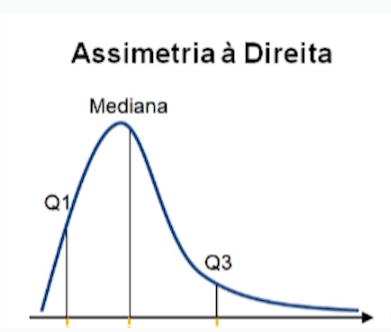
\includegraphics[width=0.5\linewidth]{dist1.png}
\end{figure}
\begin{block}{Comportamento}
 Na assimétrica a direita, a média é puxada para cima por outliers, enquanto a mediana permanece mais representativa do comportamento típico.    
\end{block}
\end{frame}

\begin{frame}{Distribuições :Normal}
    \begin{figure}
\centering
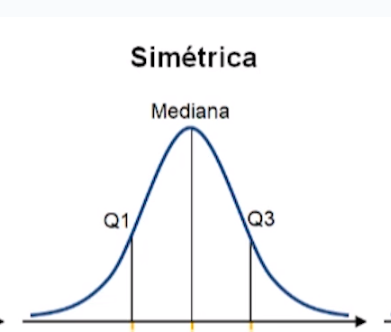
\includegraphics[width=0.5\linewidth]{dist2.png}
\end{figure}
\begin{block}{Comportamento}
 Na simetrica normal, a média e a mediana são iguais, e ambos representam bem o comportamento típico.   
\end{block}
\end{frame}
\begin{frame}{Distribuições :Assimétrica a Esquerda}
    \begin{figure}
\centering
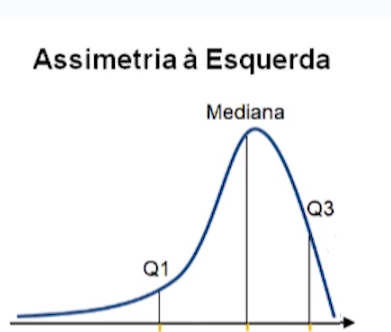
\includegraphics[width=0.5\linewidth]{dist3.png}
\end{figure}
\begin{block}{Comportamento}
Na assimétrica a esquerda, a média é puxada para baixo por outliers, enquanto a mediana permanece mais representativa do comportamento típico. 
\end{block}

\end{frame}

\begin{frame}{Box plots o que é }
    \begin{figure}
\centering
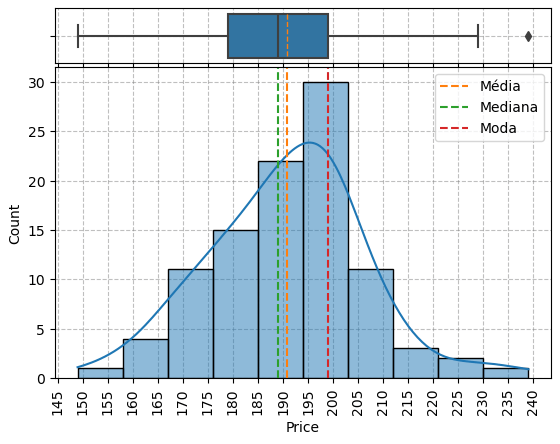
\includegraphics[width=0.65\linewidth]{Boxplots-com-Histogramas-2.png}
\end{figure}
\begin{block}{Comportamento}
O box plot mostra a mediana, os quartis e os outliers, permitindo uma visualização rápida da distribuição dos dados.
\end{block}
\end{frame}  


\begin{frame}{Box plots o que é }
    \begin{figure}
\centering
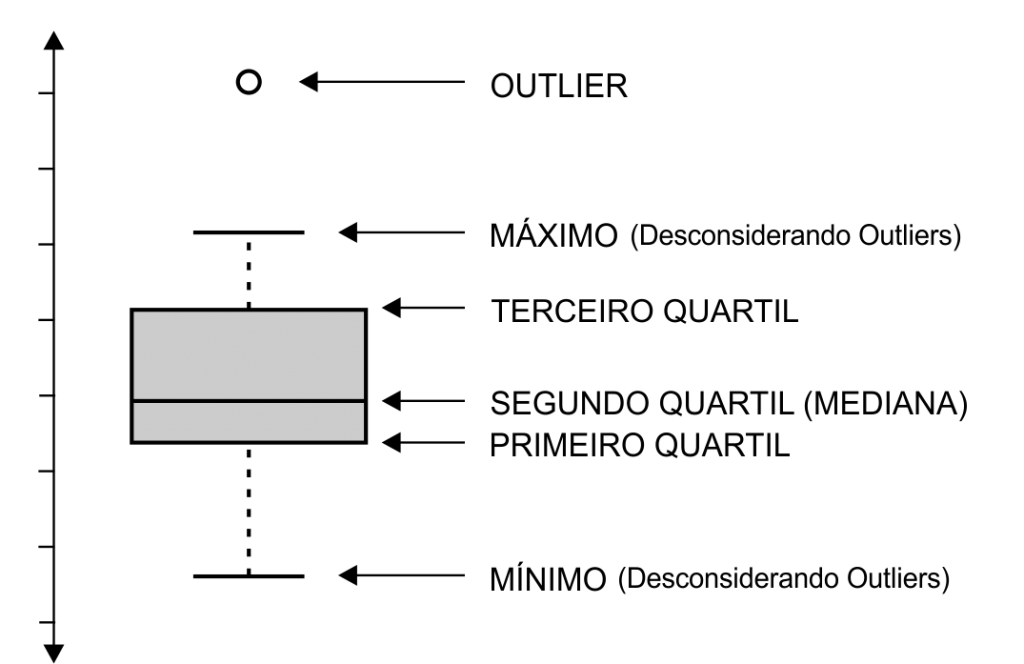
\includegraphics[width=\linewidth]{50.png}
\end{figure}
\end{frame}  


\begin{frame}{Box plots o que é }
    \begin{figure}
\centering
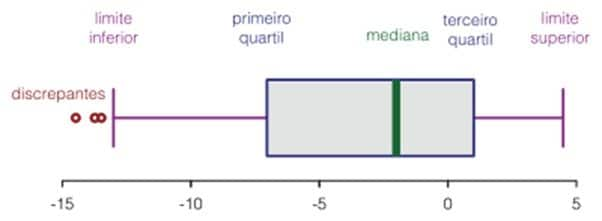
\includegraphics[width=\linewidth]{fig1.jpeg    }
\end{figure}
\end{frame}  
\begin{frame}{Box plots o que é }
    \begin{figure}
\centering
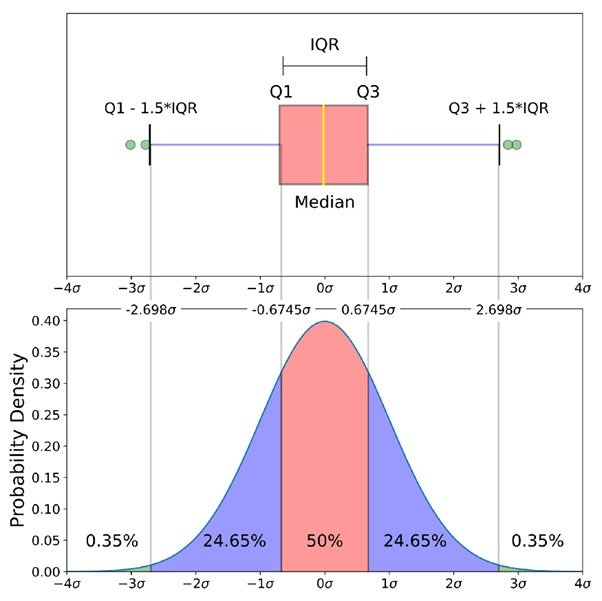
\includegraphics[width=0.65\linewidth]{FIG3.jpeg  }
\end{figure} 
\end{frame}  
\begin{frame}{Visualização: Séries Temporais}
\begin{center}
\begin{tikzpicture}
\begin{axis}[
    width=8cm, height=4cm,
    xlabel=Tempo, ylabel=Requisições,
    domain=0:10, samples=100,
    axis lines=left, xtick=\empty, ytick=\empty
]
\addplot[blue, thick] {exp(-0.5*(x-5)^2) + 0.2*rand};
\end{axis}
\end{tikzpicture}
\end{center}
\begin{itemize}
    \item Veja padrões semanais e sazonais.
\end{itemize}
\end{frame}
\begin{frame}[fragile]{Verificando Latência com Percentis}
\begin{block}{Objetivo}
Calcular os percentis de latência (P98 e P99) de um conjunto de requisições.
\end{block}

\begin{lstlisting}[language=Python]
import numpy as np

# Latencias simuladas (em ms)
latencias = np.random.normal(200, 40, 1000)

# Percentis
p98 = np.percentile(latencias, 98)
p99 = np.percentile(latencias, 99)

print("Latencia P98:", p98)
print("Latencia P99:", p99)
\end{lstlisting}

\begin{itemize}
\item Cada valor representa o tempo de resposta de uma requisição.
\item Percentis mostram o comportamento da cauda da distribuição.
\end{itemize}

\end{frame} 
\begin{frame}{Percentis de Latência}

\begin{center}
\begin{tikzpicture}[scale=0.9]

\draw[->] (0,0) -- (10,0) node[right]{Latência (ms)};
\draw[->] (0,0) -- (0,4) node[above]{Frequência};

\draw[thick]
(0.5,0) .. controls (2,3) .. (4,2)
.. controls (6,1) .. (9,0.2);

\draw[dashed] (7.2,0) -- (7.2,2);
\node[below] at (7.2,0){P98};

\draw[dashed] (8.2,0) -- (8.2,1.2);
\node[below] at (8.2,0){P99};

\end{tikzpicture}
\end{center}

\begin{block}{Interpretação}
\begin{itemize}
\item \textbf{P98}: 98\% das requisições respondem antes desse tempo.
\item \textbf{P99}: 99\% das requisições respondem antes desse tempo.
\end{itemize}
\end{block}

\begin{alertblock}{Importante em Sistemas Distribuídos}
Percentis altos revelam problemas de desempenho que a média esconde.
\end{alertblock}

\end{frame}
\begin{frame}{Distribuição de Latência}

\begin{center}
\begin{tikzpicture}

\draw[->] (0,0) -- (10,0) node[right]{Latência (ms)};
\draw[->] (0,0) -- (0,4) node[above]{Frequência};

\draw[thick,blue] plot[smooth] coordinates
{(0.5,0.3) (1.5,1.2) (2.5,2.5) (3.5,3.2) (4.5,2.6) (5.5,1.8) (6.5,1.0) (7.5,0.5) (8.5,0.2)};

\draw[dashed] (7.2,0) -- (7.2,2.0);
\node[below] at (7.2,0) {P98};

\draw[dashed] (8.0,0) -- (8.0,1.5);
\node[below] at (8.0,0) {P99};

\end{tikzpicture}
\end{center}

\begin{block}{Ideia}
Em sistemas distribuídos, analisamos a distribuição das latências para
identificar valores extremos que afetam os usuários.
\end{block}

\end{frame}
\begin{frame}{Percentil 98 e 99}

\begin{center}
\begin{tikzpicture}

\draw[->] (0,0) -- (10,0) node[right]{Latência ordenada};

\draw (1,0.4) rectangle (7.2,1);
\node at (4,1.3){98\% das requisições};

\draw (7.2,0.4) rectangle (8.0,1);
\node at (7.6,1.3){1\%};

\draw (8.0,0.4) rectangle (9.5,1);
\node at (8.8,1.3){1\%};

\draw[dashed] (7.2,0) -- (7.2,1);
\node[below] at (7.2,0){P98};

\draw[dashed] (8.0,0) -- (8.0,1);
\node[below] at (8.0,0){P99};

\end{tikzpicture}
\end{center}

\begin{itemize}
\item \textbf{Percentil 98 (P98)}: 98\% das requisições são mais rápidas que esse valor.
\item \textbf{Percentil 99 (P99)}: 99\% das requisições são mais rápidas que esse valor.
\item O 1\% restante representa as requisições mais lentas.
\end{itemize}

\end{frame}
\begin{frame}[fragile]{Cálculo dos Percentis em Python}

\begin{block}{Exemplo de cálculo}
\end{block}

\begin{lstlisting}[language=Python]

import numpy as np

# latencias simuladas em ms
latencias = np.random.normal(200, 40, 1000)

# calculo dos percentis
p98 = np.percentile(latencias, 98)
p99 = np.percentile(latencias, 99)

print("Latencia P98:", p98)
print("Latencia P99:", p99)

\end{lstlisting}

\begin{block}{Interpretação}
Se P99 = 420 ms, então 99% das requisições são respondidas em menos de 420 ms.
\end{block}

\end{frame}
\begin{frame}{Percentis de Latência}

\begin{block}{Definição}
O percentil $P_k$ é o valor abaixo do qual estão $k\%$ dos dados de uma distribuição ordenada.
\end{block}

\begin{center}
\begin{tikzpicture}

\draw[->] (0,0) -- (10,0) node[right] {Latência (ms)};

\draw[fill=blue!20] (0,0) rectangle (8.8,0.6);
\draw[fill=red!20] (8.8,0) rectangle (10,0.6);

\draw[dashed, thick] (8.8,0) -- (8.8,1.2);

\node at (4.4,0.9) {98\% das requisições};
\node at (9.4,0.9) {2\% mais lentas};

\node at (8.8,1.4) {$P_{98}$};

\end{tikzpicture}
\end{center}

\begin{alertblock}{Interpretação}
Se $P_{98} = 320\,ms$, então 98\% das requisições possuem latência menor ou igual a 320 ms.
\end{alertblock}

\end{frame} 



% -------------------------------------------------------
% SEÇÃO 7: PAINÉIS E DEBUGGING
% -------------------------------------------------------
\section{Dashboards e Processo}

\begin{frame}{O Painel SRE Ideal}
\begin{itemize}
    \item No topo: Disponibilidade global e SLO.
    \item Abaixo: Os 4 Sinais de Ouro.
    \item Mais abaixo: Links para playbooks e logs detalhados.
\end{itemize}
\end{frame}

\begin{frame}{Playbooks (Manual de Resposta)}
Cada alerta deve ter um link para um \textbf{Playbook}.
\begin{itemize}
    \item O que este alerta significa?
    \item Quais são os primeiros passos de diagnóstico?
    \item Quem contatar se escalar?
\end{itemize}
\end{frame}
\begin{frame}{Alertas do Google}
\begin{figure} 
\centering
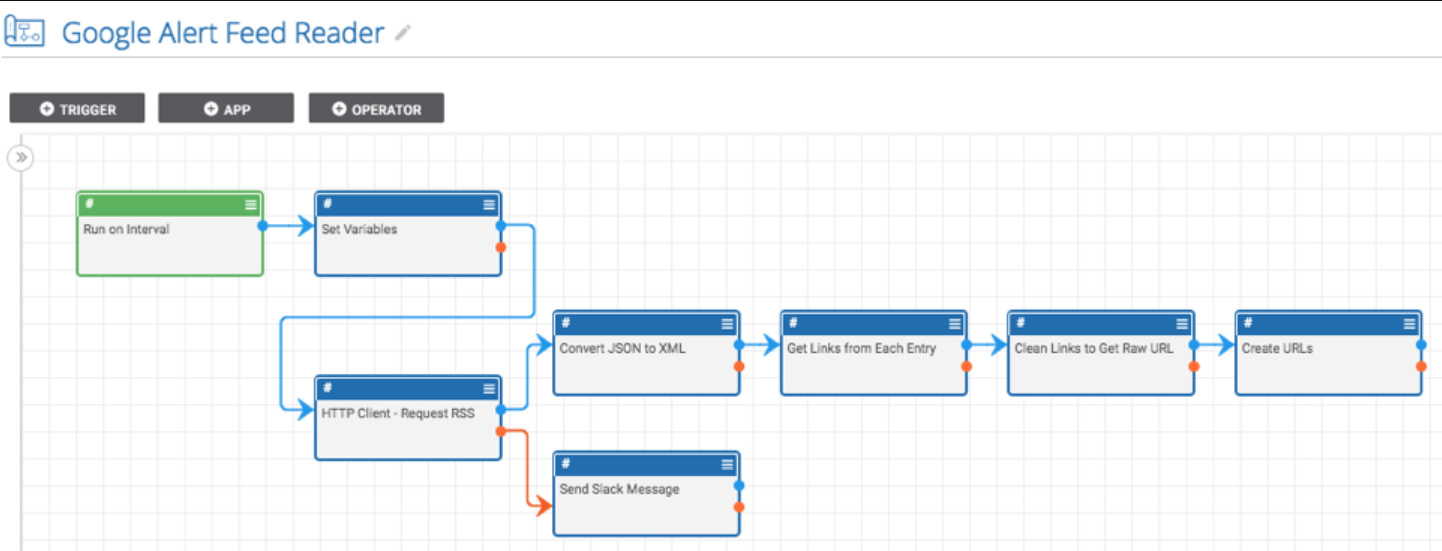
\includegraphics[width=\linewidth]{googleAlerts.png}
\caption{Alertas do Google}
\end{figure}
\end{frame}

% -------------------------------------------------------
% CONCLUSÃO
% -------------------------------------------------------
\section{Conclusão}

\begin{frame}{Conclusões Finais}
\begin{itemize}
    \item Comece simples, foque no usuário.
    \item Alerte sobre \textbf{Sintomas}.
    \item Use \textbf{Métricas de Caixa-Branca} para rapidez.
    \item Monitore para \textbf{aprender}, não apenas para consertar.
\end{itemize}
\end{frame}

\begin{frame}{Perguntas?}
\centering
\LARGE Obrigado! \\
\vspace{1cm}
\normalsize Professor Sergio Souza Novak \\
Engenharia de Qualidade e Confiabilidade
\end{frame}

\end{document}
